\author{Andrei Tkachuk}

\section{Отыскание max и min значений для ФНП}

\begin{Example}
    Найти экстремумы для функции $u = x^2 + y^2$ ограниченной поверхностью $D: |x|+2|y| \leqslant 5$
    \begin{figure}[h!]
        \noindent\centering{
            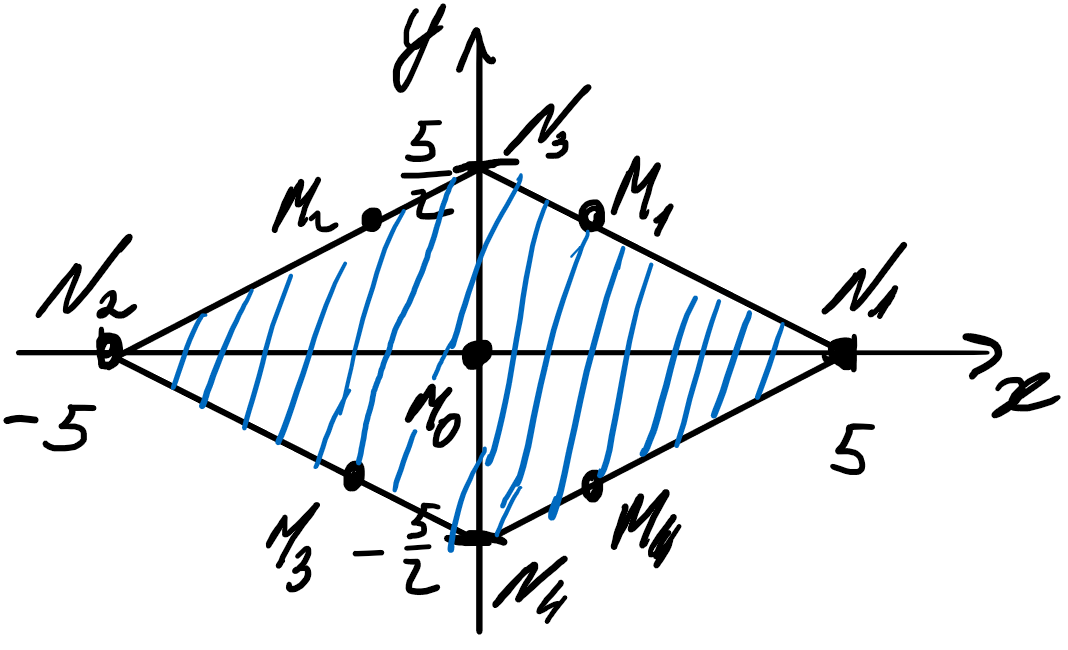
\includegraphics[width=50mm]{1_4_1.png}
            \caption{}
        }
    \end{figure}\\
    Таким образом, мы имеем дело с компактом (огр. множеством).
    \begin{enumerate}
        \item $u'_x = 2x = 0, \; u'_y = 2y = 0$\\
              $M_0(0, 0), \; u(M_0) = 0$ --- минимум
        \item Для удобства будем рассматривать первую четверть, так как компакт представляет собой ромб, который симметричен относительно осей (Замечание. Облатсть определена через 4 дифференцируемые функции).
        \begin{align*}
            &L_1 = x^2 + y^2 + \lambda(x + 2y - 5)\\
            &dL_1 = (2x + \lambda)dx + (2y + 2\lambda)dy + (x + 2y - 5)d\lambda = 0\\
            &\begin{cases}
                2x + \lambda = 0, \; x = -\frac{\lambda}{2}\\
                2y + 2\lambda = 0, \; y = -\lambda\\
                x + 2y = 5
            \end{cases}
        \end{align*}
        Подставим значения $x$ и $y$ в последнее уравнение, получим
        \[
            \lambda = -2
        \]
        следовательно экстремум в точке $M_1(1, 2)$\\
        Так как мы рассматриваем первую четветь, то в оставшихся трёх получим $M_2(-1, 2), \; M_3(-1, -2), \; M_4(1, -2)$\\
        Для данных точек значение функции 
        \[
            u(M_{1,2,3,4}) = 1 + 4 = 5
        \]
        \item Так как функция компакта не является гладкой, то рассмотрим следующие точки:
        \begin{align*}
            &N_1(5, 0), \; N_2(-5, 0) &N_3(0, \frac{5}{2}), \; N_4(0, -\frac{5}{2})\\
            &u(N_{1,2}) = 25  &u(N_{3,4}) = \frac{25}{4}
        \end{align*}
        Таким образом $u_{max} = u(N_{1,2}) = 25$.\\
        Окончательный ответ:
        \[
            \forall(x, y) \in D, \; 0 \leqslant u(x, y) \leqslant 25
        \]
    \end{enumerate}
\end{Example}

\begin{Note}[Как выглядит в общем случае]
    Пусть $u = f(x_1, \dots, x_n)$ определена в замкнутой односвязанной области $D : \varphi_1(M) \geqslant 0, \dots, \varphi_k(M) \geqslant 0$
    \begin{enumerate}
        \item $M \in \mathring{D}: \varphi_1(M) > 0, \dots, \varphi_k(M) > 0$\\
        Должно соблюдаться $f(M),\; \varphi_1(M),\; \dots,\; \varphi_k(M) \in C'(\mathring{D})$ --- гладкая по каждой части границы\\
        Для $df(M) = 0 \; \exists M_1, \dots, M_l \in \mathring{D}$ --- гладкая n-мерная часть
        
        \item Гладкая $(n-1)$ мерная часть границы $D$
        \begin{align*}
            &L_1 = f + \lambda_1\varphi_1&, &\dots,& &L_k = f + \lambda_k\varphi_k\\
            &dL_1 = 0& && & dL_k = 0\\
            &N_{1 1}, \dots, N_{1 l_1} + \lambda& && &N_{1 1}, \dots, N_{1 l_k} + \lambda
        \end{align*}
        $\varphi_1(N_{1 1}) = 0, \varphi_2(N_{1 1}) > 0, \dots, \varphi_k(N_{1 1}) > 0$
            
        \item Гладкая $(n-2)$ мерная часть границы $D$. Рассмотрим функции вида
        \[
            L = f(M) + \lambda_i\,\varphi_i(M) + \lambda_j\,\varphi_j(M)
        \]
        \begin{align*}
            S: &\varphi_i(M) = 0, &\varphi_j(M) = 0 \qquad (i \neq j)\\ 
            &1 \leqslant i \leqslant k  &1 \leqslant j \leqslant k\\
        \end{align*}
        Рассматриваем
        \[
            dL(M, \lambda_i, \lambda_j) = 0
        \]
        Получаем следующий набор точек $K_1,\; \dots,\; K_s$
        
        \item [\dots)]
        
        \item [n + 1)] Рассматриваем 0-мерное гладкое пространство (вершины или "плохие" точки). Получим следующее множетсво: $P_1,\; \dots,\; P_q$
    \end{enumerate}
    Таким образом, ответ:
    \begin{align*}
        U_{max} &= max\{u(M_1), \; \dots, \; u(P_q)\}\\
        U_{min} &= min\{u(M_1), \; \dots, \; u(P_q)\}
    \end{align*}
\end{Note}
\textcolor{cyan}{Тут надо написать обощающий алгоритм, т.е. что по факту для поиска экстремумов мы рассматриваем множества различных функций Лагранжа для различного количества границ.}